\section{Supplementary Materials for Section~\ref{section:experiments}}
\label{section:supp-to-experiment}


To better understand how each algorithm works, we plot in
Figure~\ref{fig:banditron-points},~\ref{fig:linearova-points},~\ref{fig:rationalova-points}
the final decision boundary that is learned by each algorithm.

\begin{figure}[h!]
    \centering
    \begin{subfigure}[b]{0.23\textwidth}
        \captionsetup{justification=centering}
        \begin{center}
        \hspace*{-0.3cm} 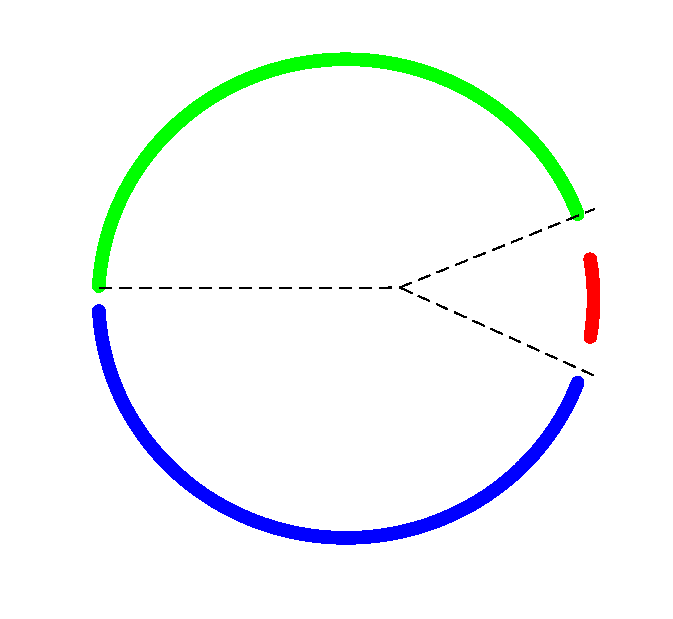
\includegraphics[width=1.15\textwidth, trim={0, 0cm, 0, 0}, clip]{figures/strong_banditron_points}
        \caption{Strongly separable case}
        \end{center}
    \end{subfigure}
    \hfill
    \begin{subfigure}[b]{0.23\textwidth}
        \captionsetup{justification=centering}
        \centering
        \hspace*{-0.3cm}  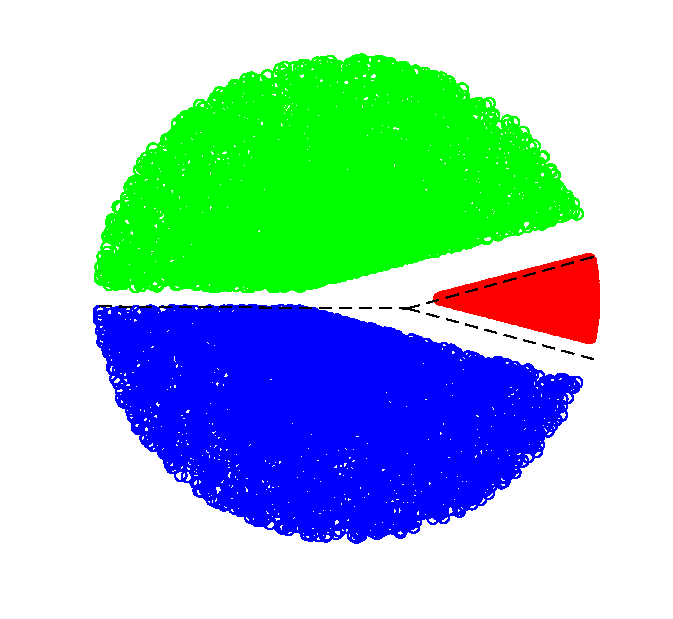
\includegraphics[width=1.15\textwidth, trim={0, 0cm, 0, 0}, clip]{figures/weak_banditron_points}
         \caption{Weakly separable case}
    \end{subfigure}
    \vspace*{-0.2cm}
    \caption{\textsc{Banditron}'s decision boundary}
     \label{fig:banditron-points}
\end{figure}

\begin{figure}[h!]
    \centering
    \begin{subfigure}[b]{0.23\textwidth}
        \captionsetup{justification=centering}
        \begin{center}
        \hspace*{-0.3cm} 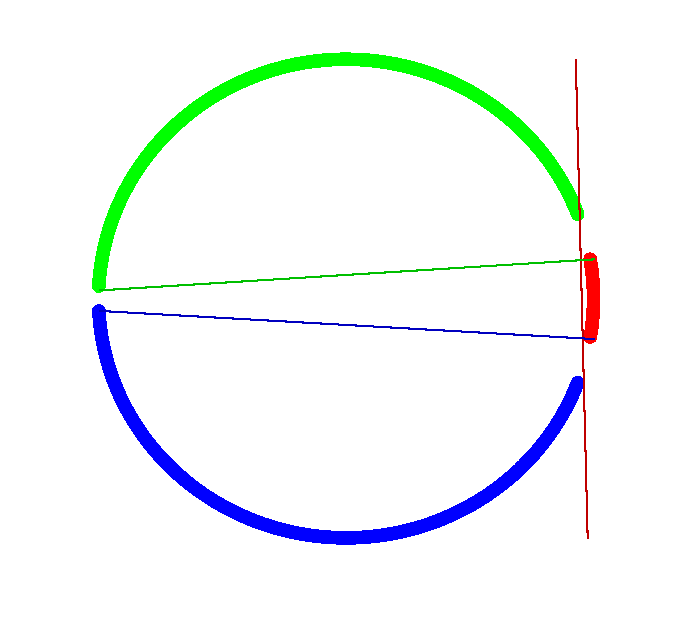
\includegraphics[width=1.15\textwidth, trim={0, 0cm, 0, 0}, clip]{figures/strong_linear_ova_points}
        \caption{Strongly separable case}
        \end{center}
    \end{subfigure}
    \hfill
    \begin{subfigure}[b]{0.23\textwidth}
        \captionsetup{justification=centering}
        \centering
        \hspace*{-0.3cm}  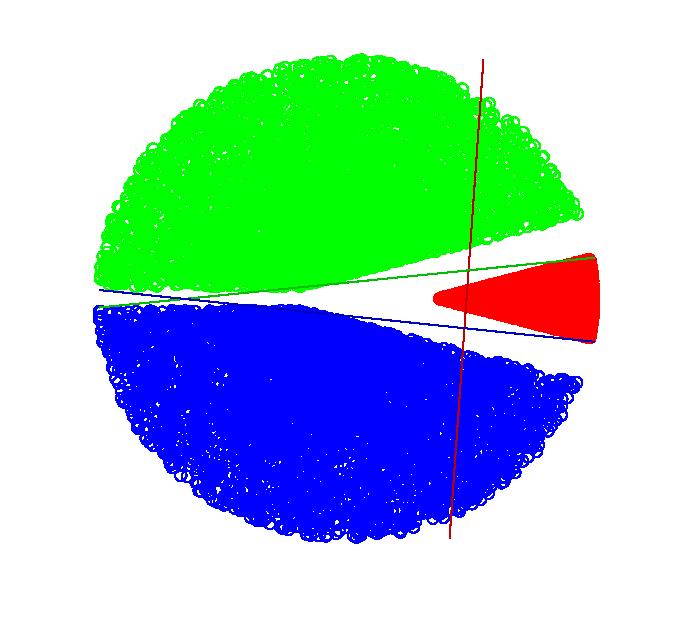
\includegraphics[width=1.15\textwidth, trim={0, 0cm, 0, 0}, clip]{figures/weak_linear_ova_points}
         \caption{Weakly separable case}
    \end{subfigure}
    \vspace*{-0.2cm}
    \caption{Our Algorithm with linear kernel (Algorithm~\ref{algorithm:algorithm-for-strongly-linearly-separable-examples})'s decision boundary}
    \label{fig:linearova-points}
\end{figure}

\begin{figure}[h!]
    \centering
    \begin{subfigure}[b]{0.23\textwidth}
        \captionsetup{justification=centering}
        \begin{center}
        \hspace*{-0.3cm} 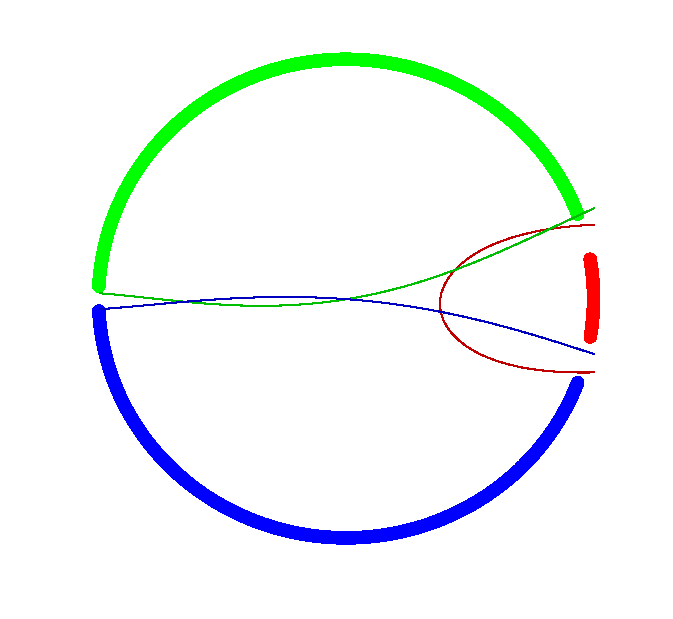
\includegraphics[width=1.15\textwidth, trim={0, 0cm, 0, 0}, clip]{figures/strong_rational_ova_points}
        \caption{Strongly separable case}
        \end{center}
    \end{subfigure}
    \hfill
    \begin{subfigure}[b]{0.23\textwidth}
        \captionsetup{justification=centering}
        \centering
        \hspace*{-0.3cm}  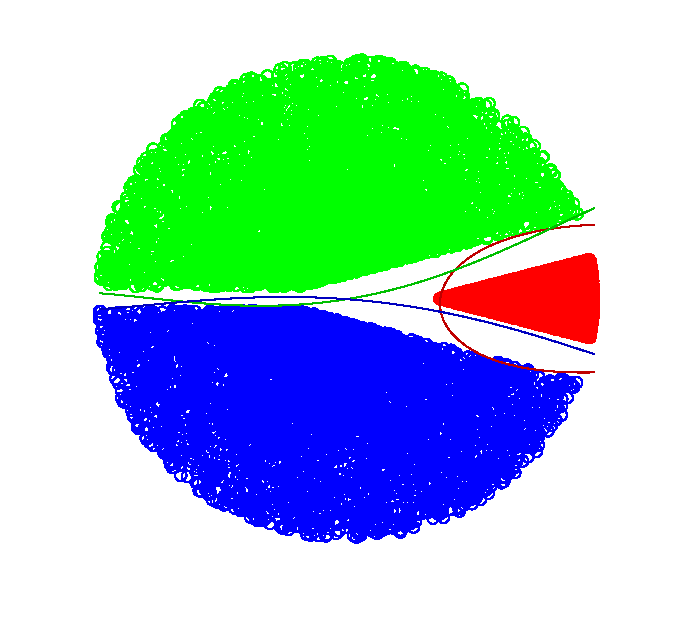
\includegraphics[width=1.15\textwidth, trim={0, 0cm, 0, 0}, clip]{figures/weak_rational_ova_points}
         \caption{Weakly separable case}
    \end{subfigure}
    \vspace*{-0.2cm}
    \caption{Our Algorithm with rational kernel (Algorithm~\ref{algorithm:kernelized})'s decision boundary}
    \label{fig:rationalova-points}
\end{figure}
